\documentclass[a4paper,12pt]{article}
\usepackage[utf8]{inputenc} % mã hóa UTF-8
\usepackage[T5]{fontenc}    % font cho tiếng Việt
\usepackage[vietnamese]{babel} % hỗ trợ tiếng Việt
\usepackage{graphicx}
\usepackage[svgnames]{xcolor}
\usepackage{xcolor}
\usepackage{listings}
\usepackage{tocloft}
\usepackage{hyperref}
\usepackage{enumitem}
\usepackage{float}

\graphicspath{{data/}}

% Cấu hình hiển thị code Python
\lstset{
    basicstyle=\ttfamily\small,
    keywordstyle=\color{blue}\bfseries,
    stringstyle=\color{red},
    commentstyle=\color{green!60!black}\itshape,
    numbers=left,
    numberstyle=\tiny,
    stepnumber=1,
    numbersep=5pt,
    showspaces=false,
    showstringspaces=false,
    frame=single,
    breaklines=true,
    breakatwhitespace=true,
    tabsize=4,
    language=Python
}

% Cấu hình mục lục
\renewcommand{\cftsecleader}{\cftdotfill{\cftdotsep}}
\setlength{\cftbeforesecskip}{5pt}
\setlength{\cftbeforesubsecskip}{2pt}

% Thông tin tài liệu
\title{\textbf{Hướng Dẫn Sử Dụng Chương Trình Bài Tập Giữa Kỳ}}

\author{
    \textbf{Nhóm Thực Hiện} \\[12pt]
    \begin{tabular}{c}
        Trần Huỳnh Trung Hiếu \\ MSSV: N21DCCN122 \\[8pt]
        Nguyễn Thị Thanh Huyến \\ MSSV: N21DCCN130 \\[8pt]
        Nguyễn Thị Huyền My \\ MSSV: N21DCCN47 \\[8pt]
        Tô Phan Kiều Thương \\ MSSV: N21DCCN184 \\[12pt]
        \textit{Khoa Công Nghệ Thông Tin,} \\
        \textit{Học Viện Công Nghệ Bưu Chính Viễn Thông Cơ Sở TP.HCM}
    \end{tabular}
}


\date{Tháng 5, 2025}

\begin{document}

\maketitle
\thispagestyle{empty}
\newpage

\tableofcontents
\newpage

\section{Giới thiệu}
Chương trình \textbf{Object Image Editor} là một ứng dụng giao diện đồ họa (GUI) được phát triển bằng Python, sử dụng thư viện \texttt{tkinter} và \texttt{PIL} để quản lý và chỉnh sửa các ảnh chứa các object hình chữ nhật. Chương trình cho phép người dùng thêm ảnh, chỉnh sửa object, áp dụng các phép biến đổi, chuyển đổi object giữa các ảnh, và tạo chuỗi biến đổi với tính toán chi phí. Ứng dụng được thiết kế với giao diện trực quan, sử dụng màu nền \texttt{\#f0f4f8}, font \texttt{Helvetica}, và các canvas có thanh cuộn để hiển thị ảnh. Giao diện chính bao gồm nhiều tab chức năng: Home, Transformation Library Manager (TLM), Cost Function Server (CFS), Object Convertor (OC), Sequence Editor, và About.

Mục tiêu của chương trình là cung cấp một công cụ linh hoạt để thao tác trên các ảnh và object, đồng thời hỗ trợ tính toán chi phí cho các phép biến đổi, phù hợp với các yêu cầu xử lý ảnh cơ bản trong học thuật và thực tiễn.

\section{Cấu trúc chương trình}
Chương trình được tổ chức thành nhiều module, mỗi module đảm nhận một chức năng cụ thể:

\begin{itemize}
    \item \textbf{\texttt{main.py}}: Tệp chính, khởi tạo giao diện với \texttt{ttk.Notebook} chứa các tab: Home, TLM, CFS, OC, Sequence Editor, About.
    \item \textbf{\texttt{tab/Home\_tab.py}}: Quản lý hiển thị ảnh, thêm ảnh mới, và chỉnh sửa object (tọa độ, màu RGB).
    \item \textbf{\texttt{tab/TLM\_tab.py}}: Quản lý thư viện phép biến đổi, hỗ trợ áp dụng toán tử từ JSON hoặc nhập thủ công.
    \item \textbf{\texttt{tab/CFS\_tab.py}}: Quản lý hàm chi phí, đọc và ghi vào \texttt{cost\_functions.json}.
    \item \textbf{\texttt{tab/OC\_tab.py}}: Chuyển đổi object giữa hai ảnh, tính toán chuỗi biến đổi và chi phí.
    \item \textbf{\texttt{tab/Sequence\_tab.py}}: Tab Sequence Editor, cho phép tạo và áp dụng chuỗi biến đổi trên các object.
    \item \textbf{\texttt{object\_manager.py}}: Quản lý cơ sở dữ liệu ảnh (\texttt{ImageDatabase}) và các object (\texttt{ImageObjectRegion}).
    \item \textbf{\texttt{transformation\_manager.py}}: Quản lý thư viện phép biến đổi (\texttt{TransformationLibraryManager}).
    \item \textbf{\texttt{cost\_function\_server.py}}: Xử lý tính toán chi phí dựa trên \texttt{cost\_functions.json}.
    \item \textbf{\texttt{object\_converter.py}}: Hỗ trợ chuyển đổi object giữa hai ảnh.
    \item \textbf{\texttt{data/transformations.json}}: Lưu danh sách toán tử và tham số.
    \item \textbf{\texttt{data/cost\_functions.json}}: Lưu danh sách hàm chi phí.
\end{itemize}

\section{Yêu cầu cài đặt}
Clone dự án từ Github: \href{https://github.com/huyenmy239/transform-similarity-retrieval}{https://github.com/huyenmy239/transform-similarity-retrieval}
Để chạy chương trình, bạn cần cài đặt Python và các thư viện sau:

\begin{lstlisting}[language=bash]
pip install -r requirements.txt
\end{lstlisting}

\section{Hướng dẫn chạy chương trình}

\subsection{Chạy giao diện chính (\texttt{main.py})}
\begin{enumerate}
    \item Mở terminal (dòng lệnh) trong thư mục chứa mã nguồn.
    \item Chạy lệnh:
    \begin{lstlisting}[language=bash]
python main.py
    \end{lstlisting}
    \begin{figure}[h]
        \centering
        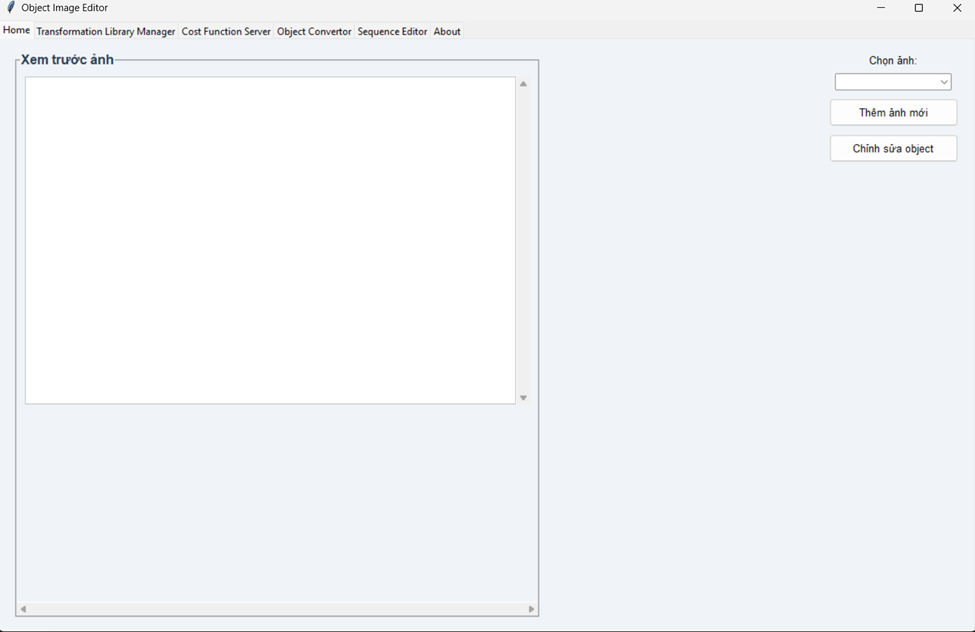
\includegraphics[width=0.8\textwidth]{home.png}
        \caption{Giao diện chính}
        \label{fig:home_tab}
    \end{figure}
    \item Giao diện chính sẽ hiện ra với 6 tab: \texttt{Home}, \texttt{Transformation Library Manager}, \texttt{Cost Function Server}, \texttt{Object Convertor}, \texttt{Sequence Editor}, \texttt{About}.
    \item Thực hiện theo hướng dẫn trong từng tab để sử dụng các chức năng:
    \begin{itemize}
        \item \textbf{Home}: Quản lý danh sách ảnh, thêm ảnh mới, và chỉnh sửa object.
        \begin{figure}[h]
    \centering
    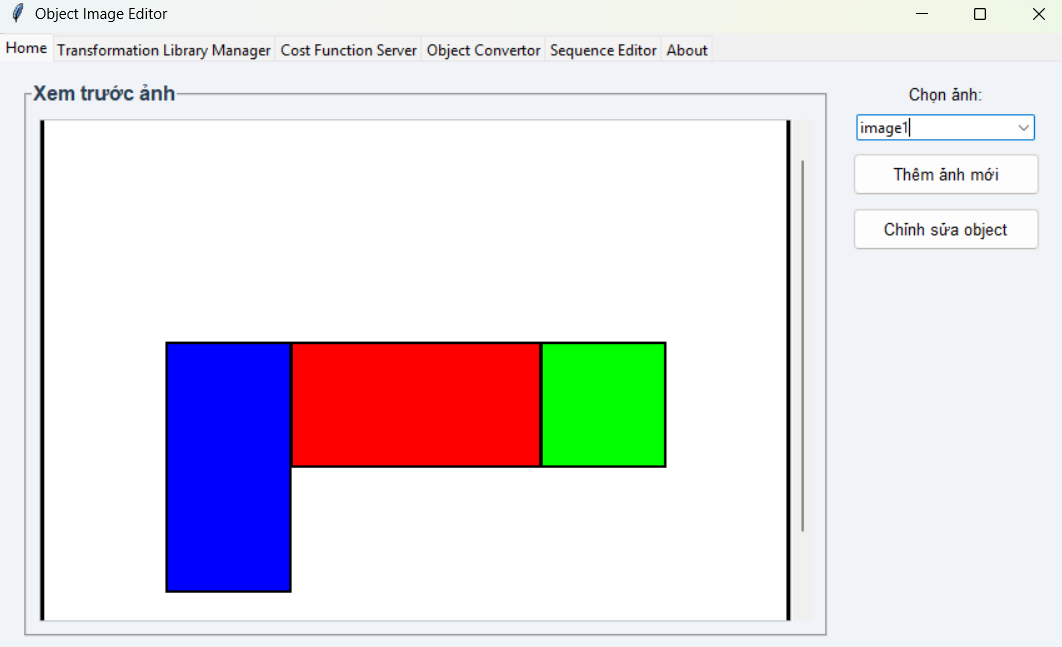
\includegraphics[width=0.8\textwidth]{home1.png}
    \caption{Giao diện home}
    \label{fig:home_tab}
\end{figure}
        \begin{enumerate}
            \item Chọn ảnh từ Combobox ``Chọn ảnh'' để xem trước trên canvas.
            \item Nhấn ``Thêm ảnh mới'', nhập tên, tọa độ ảnh (ví dụ: anh1, 0, 0, 100, 100), nhấn ``Tạo ảnh''.
            \item Nhấn ``Chỉnh sửa object'', thêm/xóa object, chỉnh sửa tọa độ (x1, y1, x2, y2) và màu RGB (ví dụ: (255,0,0)), nhấn ``Lưu''.
        \end{enumerate}
        \item \textbf{Transformation Library Manager (TLM)}: Áp dụng phép biến đổi lên object.
        \begin{figure}[H]
    \centering
    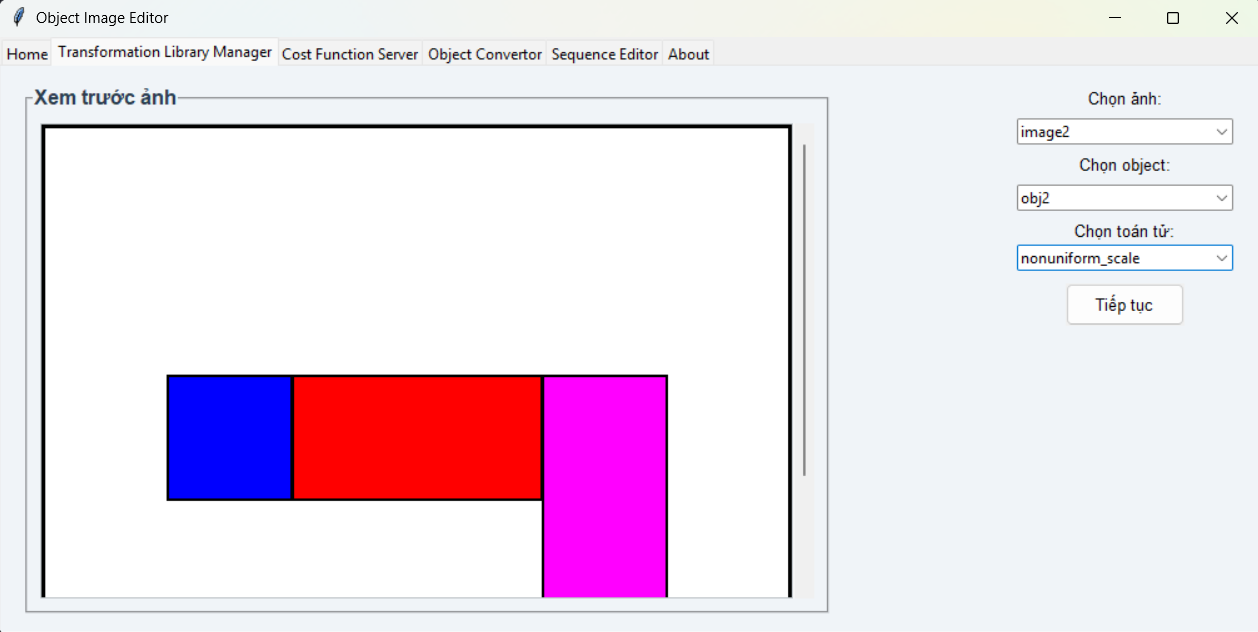
\includegraphics[width=0.8\textwidth]{TLM.png}
    \caption{Giao diện tab Transformation Library Manager}
    \label{fig:tlm_tab}
\end{figure}
        \begin{enumerate}
            \item Chọn ảnh từ Combobox ``Chọn ảnh'' để hiển thị trên canvas.
            \item Chọn object từ Combobox ``Chọn object''.
            \item Chọn toán tử (ví dụ: translate, scale) từ Combobox ``Chọn toán tử'', nhấn ``Tiếp tục''.
            \item Trong cửa sổ tùy chọn, chọn:
            \begin{itemize}
                \item ``Chọn từ file JSON'': Chọn tham số từ \texttt{transformations.json} (ví dụ: \{``dx'': 10, ``dy'': 20\}), nhấn ``Áp dụng''.
                \item ``Nhập tham số thủ công'': Nhập tham số (ví dụ: dx=10, dy=20), nhấn ``Áp dụng''.
            \end{itemize}
            \item Kiểm tra canvas để xem đối tượng sau khi biến đổi.
        \end{enumerate}
        \item \textbf{Cost Function Server (CFS)}: Quản lý và tính toán hàm chi phí.
        \begin{figure}[H]
    \centering
    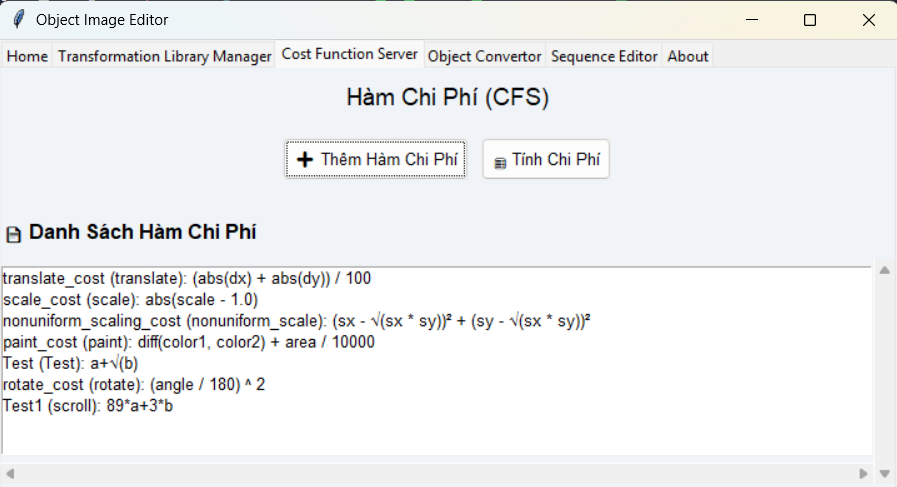
\includegraphics[width=0.8\textwidth]{CFS.png}
    \caption{Giao diện tab Cost Function Server}
    \label{fig:tlm_tab}
\end{figure}
        \begin{enumerate}
            \item Xem danh sách hàm chi phí trong Listbox.
            \item Nhấn ``Thêm Hàm Chi Phí'', nhập tên (ví dụ: translate\_cost), loại phép biến đổi (translate), công thức (ví dụ: dx + dy), sử dụng máy tính công thức, nhấn ``Xác Nhận''.
            \item Nhấn ``Tính Chi Phí'', chọn hàm chi phí, nhập tham số (ví dụ: dx=10, dy=20), nhấn ``Tính'' để xem kết quả trong messagebox.
        \end{enumerate}
        \item \textbf{Object Convertor (OC)}: Chuyển đổi object giữa hai ảnh.
        \begin{figure}[H]
    \centering
    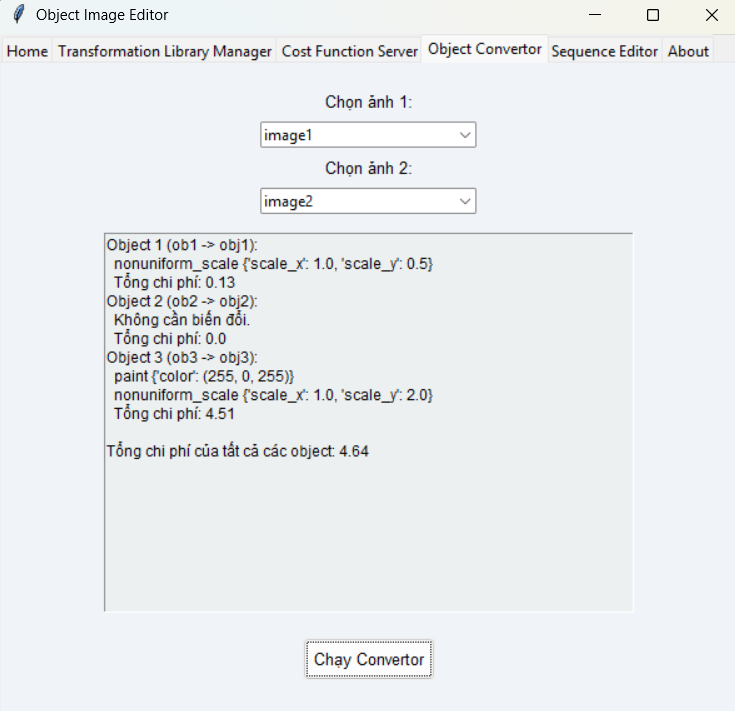
\includegraphics[width=0.8\textwidth]{OC.png}
    \caption{Giao diện tab Object Convertor}
    \label{fig:tlm_tab}
\end{figure}
        \begin{enumerate}
            \item Chọn hai ảnh từ Combobox ``Chọn ảnh 1'' và ``Chọn ảnh 2'' (ảnh 2 không trùng ảnh 1).
            \item Nhấn ``Chạy Convertor'' để xem chuỗi biến đổi và chi phí trong Text widget.
            \item Kiểm tra kết quả: chuỗi biến đổi cho từng object (ví dụ: translate \{``dx'': 10, ``dy'': 20\}) và tổng chi phí.
        \end{enumerate}
        \item \textbf{Sequence Editor}: Tạo và áp dụng chuỗi biến đổi.
        \begin{figure}[H]
    \centering
    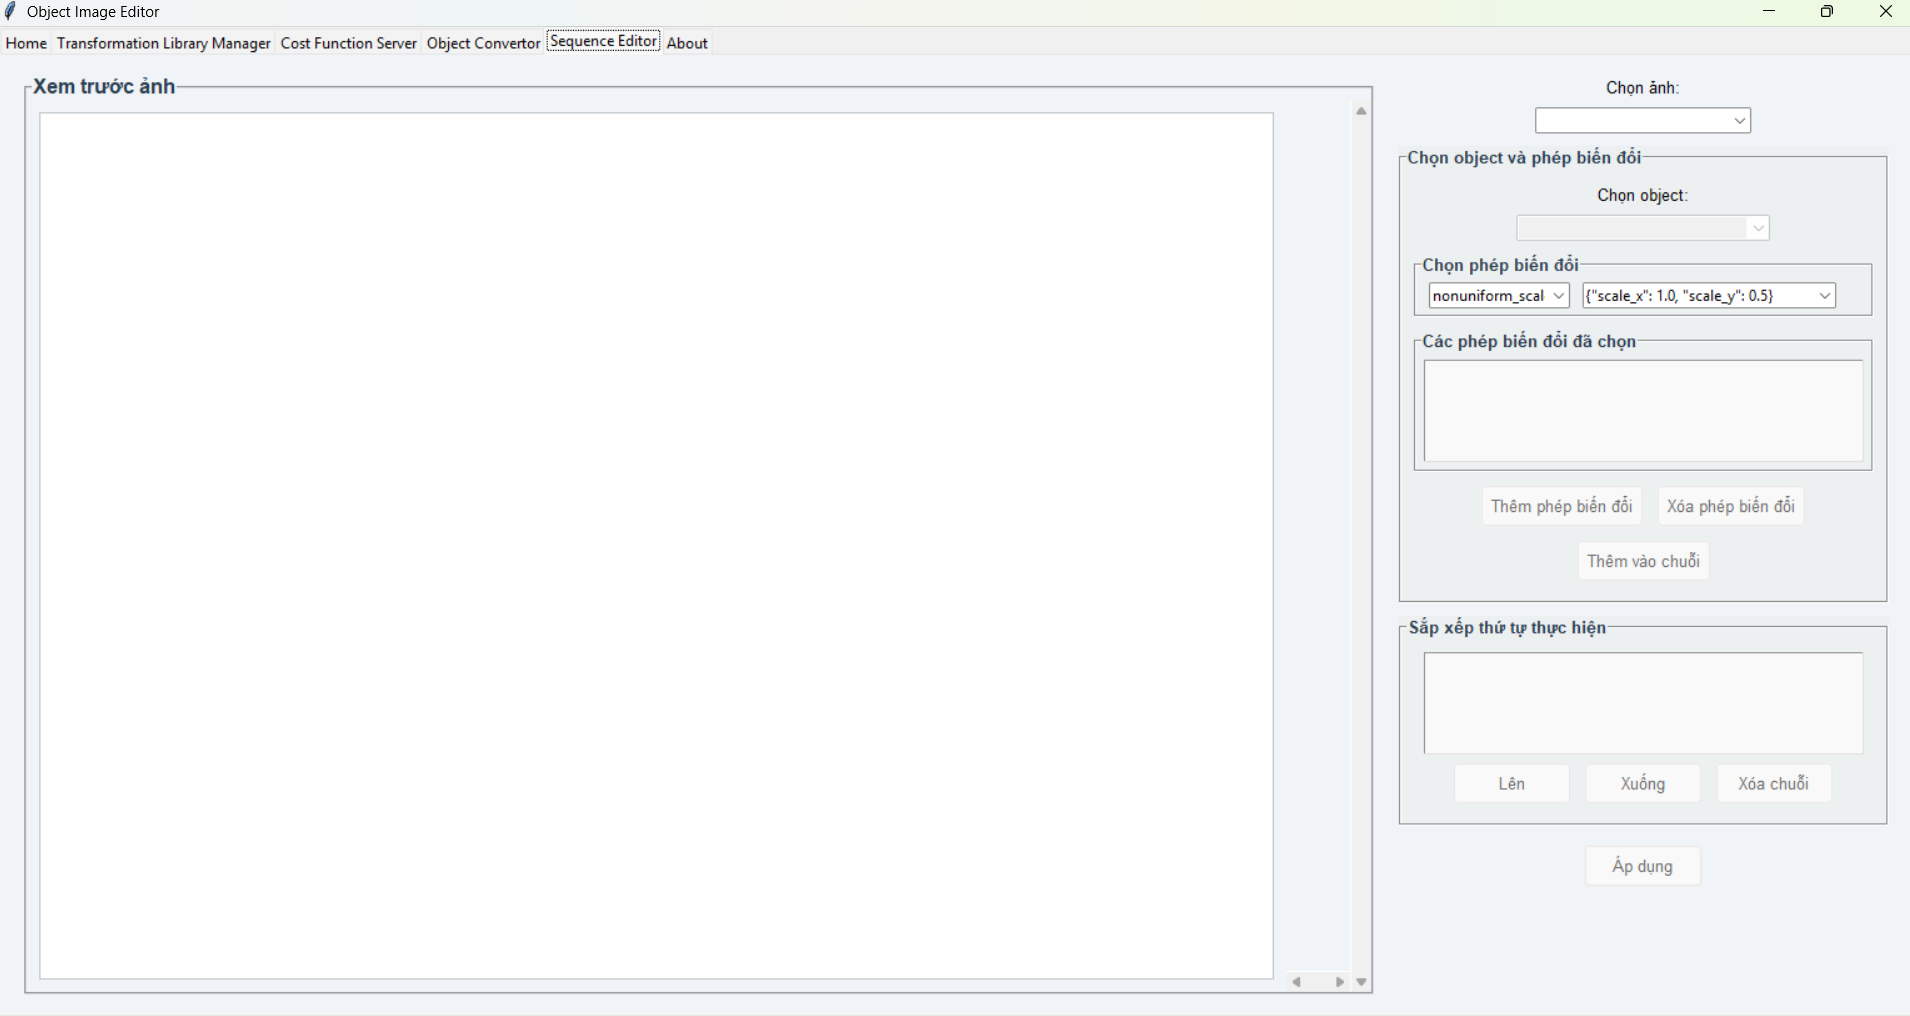
\includegraphics[width=0.8\textwidth]{SE.png}
    \caption{Giao diện tab Sequence Editor}
    \label{fig:tlm_tab}
\end{figure}
        \begin{enumerate}
            \item Chọn ảnh từ Combobox ``Chọn ảnh'' để hiển thị trên canvas.
            \item Chọn object từ Combobox ``Chọn object''.
            \item Chọn toán tử và tham số (ví dụ: translate, \{``dx'': 10, ``dy'': 20\}) từ Combobox, nhấn ``Thêm phép biến đổi'' để thêm vào Listbox tạm thời.
            \item Nhấn ``Thêm vào chuỗi'' để thêm vào Listbox chuỗi chính.
            \item Sắp xếp chuỗi bằng nút ``Lên''/``Xuống'' hoặc xóa bằng ``Xóa chuỗi''.
            \item Nhấn ``Áp dụng'' để chạy chuỗi, xem kết quả trong Text widget (giai đoạn, chi phí, lỗi nếu có).
        \end{enumerate}
        \item \textbf{About}: Xem thông tin về chương trình và tác giả.
        \begin{enumerate}
            \item Chuyển sang tab để đọc thông tin tĩnh (tên chương trình, nhóm thực hiện).
        \end{enumerate}
    \end{itemize}
\end{enumerate}

\section{Ví dụ minh họa sử dụng chương trình}

\subsection{Tạo ảnh mới}
\begin{figure}[H]
    \centering
    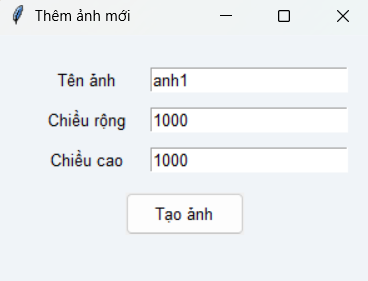
\includegraphics[width=0.8\textwidth]{addPic.png}
    \caption{Thêm ảnh mới}
    \label{fig:tlm_tab}
    \end{figure}
\begin{enumerate}
    \item Nhấn nút “Thêm ảnh mới”.
    \item Nhập tên ảnh: \texttt{anh1}, chiều rộng : \texttt{1000}, chiều cao : \texttt{1000}.
    \item Nhấn “Tạo ảnh”.
\end{enumerate}

\subsection{Thêm đối tượng}
\begin{figure}[H]
    \centering
    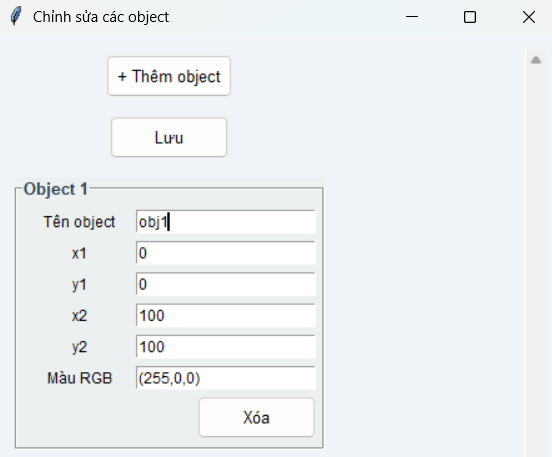
\includegraphics[width=0.8\textwidth]{addObj.png}
    \caption{Thêm đối tượng mới cho ảnh}
    \label{fig:tlm_tab}
    \end{figure}
\begin{enumerate}
    \item Chọn ảnh vừa tạo.
    \item Nhấn “Chỉnh sửa ảnh”.
    \item Nhấn “Thêm đối tượng”.
    \item Nhập tên đối tượng
    \item Nhập tọa độ đối tượng: (x1=0, y1=0, x2=100, y2=100), màu sắc: (255, 0, 0).
    \item Nhấn “Lưu”.
    \begin{figure}[H]
    \centering
    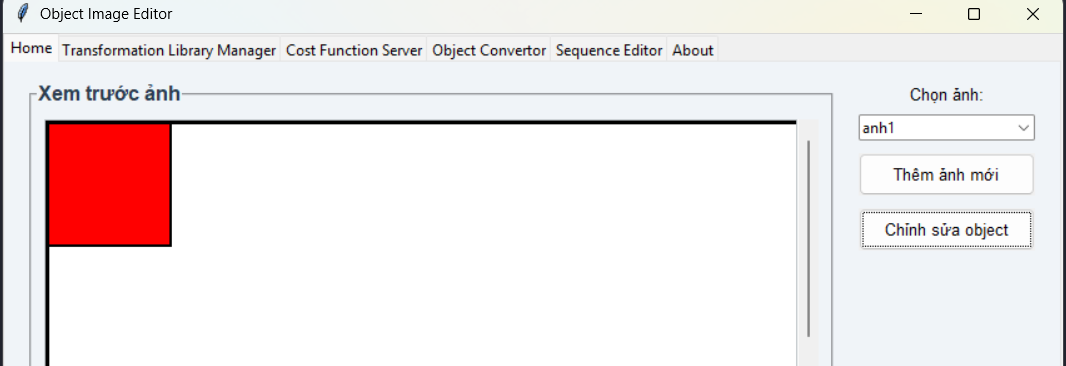
\includegraphics[width=0.8\textwidth]{affterSaveObj.png}
    \caption{Đối tượng mới được tạo thành công}
    \label{fig:tlm_tab}
    \end{figure}
\end{enumerate}

\subsection{Áp dụng biến đổi}
\begin{figure}[H]
    \centering
    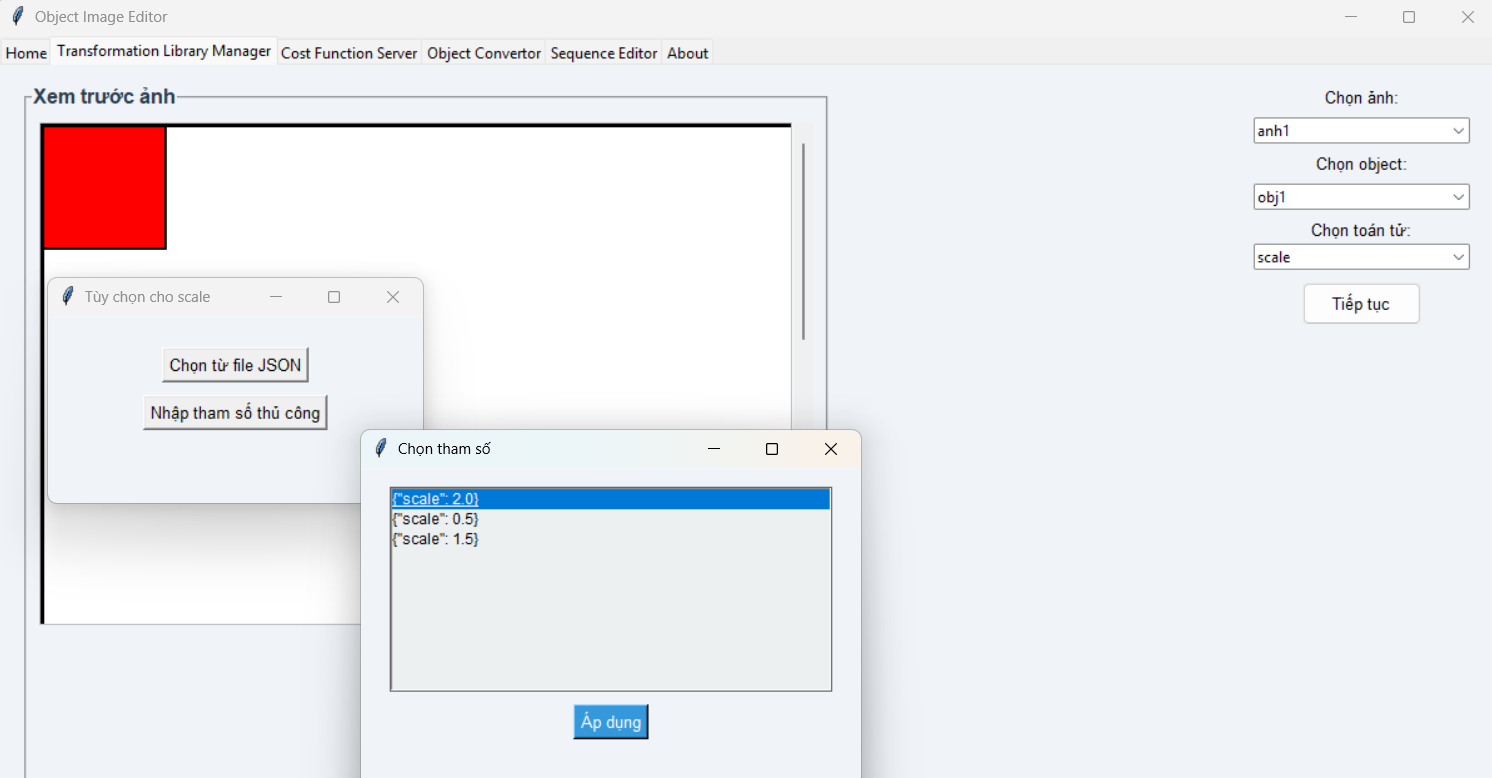
\includegraphics[width=0.8\textwidth]{Tranform.png}
    \caption{Chuyển đổi ảnh}
    \label{fig:tlm_tab}
    \end{figure}
\begin{enumerate}
    \item Chọn tab "Transformation Library Manager".
    \item Chọn ảnh có đối tượng.
    \item Nhấn “Biến đổi đối tượng”.
    \item Chọn phép biến đổi \texttt{scale}, nhấn "Tiếp tục"
    \item Nhập từ json, chọn tham số có sẵn: \texttt{{"scale":2.0}}.
    \item Nhấn “Áp dụng”.
\end{enumerate}

\subsection{Thêm Hàm Chi Phí}
\begin{figure}[H]
    \centering
    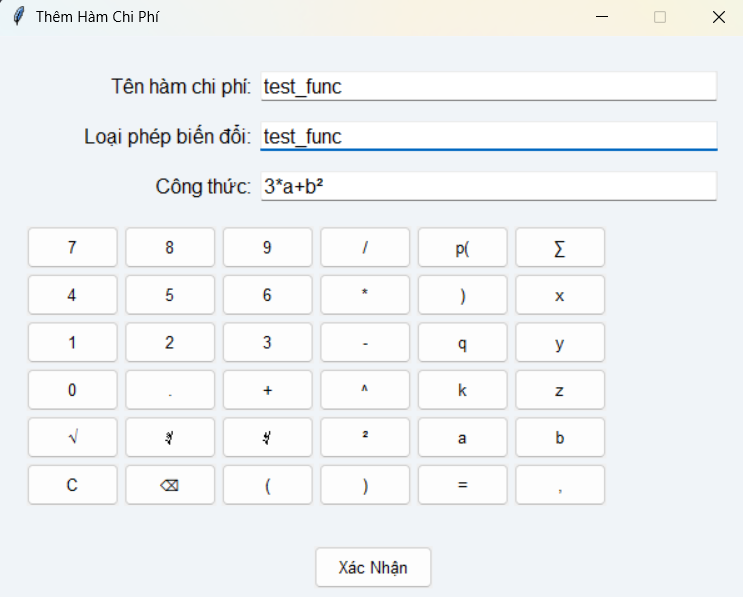
\includegraphics[width=0.8\textwidth]{addCost.png}
    \caption{Thêm mới hàm chi phí}
    \label{fig:tlm_tab}
    \end{figure}
\begin{enumerate}
    \item Chọn tab “Cost Function Server”.
    \item Nhấn “Thêm Hàm Chi Phí”.
    \item 
    \item Nhập tên hàm chi phí: \texttt{test\_func}, loại phép biến đổi: \texttt{test\_func}, công thức: \texttt{dx + dy}.
    \item Nhấn “Xác Nhận”.
\end{enumerate}
\begin{figure}[H]
    \centering
    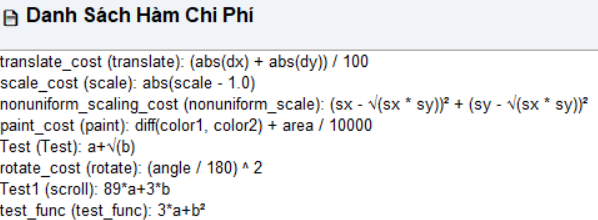
\includegraphics[width=0.8\textwidth]{afterAddCost.png}
    \caption{Hàm chi phí được thêm thành công}
    \label{fig:tlm_tab}
    \end{figure}
\subsection{Tính Chi Phí}
\begin{figure}[H]
    \centering
    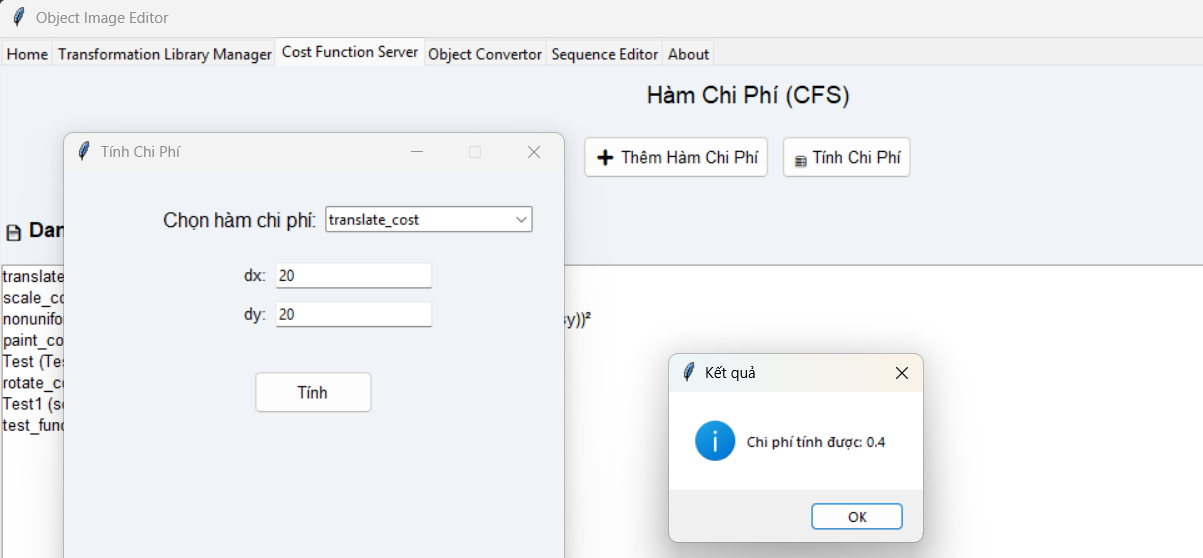
\includegraphics[width=0.8\textwidth]{eval.png}
    \caption{Tính hàm chi phí}
    \label{fig:tlm_tab}
    \end{figure}
\begin{enumerate}
    \item Nhấn “Tính Chi Phí”.
    \item Chọn hàm chi phí: \texttt{translate\_cost}.
    \item Nhập tham số: \texttt{dx=10, dy=20}.
    \item Nhấn “Tính”.
    \item Kết quả sẽ hiển thị trong messagebox.
    \end{enumerate}

\subsection{Tạo chuỗi biến đổi}
\begin{enumerate}
    \item Mở tab “Sequence Transformation”.
    \item Chọn ảnh và đối tượng.
    \item Thêm các phép biến đổi: \texttt{scale}, \texttt{rotate}, \texttt{translate}.
    \item Nhấn “Thêm vào chuỗi”.
    \item Sắp xếp chuỗi biến đổi theo thứ tự mong muốn rồi nhấn “Áp dụng”.
    \item Quan sát kết quả và chi phí trong hộp văn bản.
\end{enumerate}

\section{Tổng kết}
Chương trình \texttt{Object Image Editor} là công cụ hữu ích giúp người dùng thử nghiệm các phép biến đổi đối tượng ảnh một cách trực quan và dễ dàng. Tài liệu này cung cấp hướng dẫn chi tiết từng bước để chạy và sử dụng các chức năng chính của chương trình.

\section{Tài liệu tham khảo}
\begin{itemize}
    \item Thư viện Python: \texttt{tkinter}, \texttt{PIL}, \texttt{json}.
    \item Tài liệu LaTeX: \url{https://www.overleaf.com/learn}.
\end{itemize}

\end{document}
